%%%%%%%%%%%%%%%%%%%%%%%%%%%%%%%%%%%%%%%%%%%%%%%%
% BOZZA PER TESI DI LAUREA IN LATEX
%%%%%%%%%%%%%%%%%%%%%%%%%%%%%%%%%%%%%%%%%%%%%%%%

%\documentclass[12pt,titlepage]{book}
\documentclass[a4paper,12pt]{article}
\usepackage[british]{babel}
%\usepackage{graphics}
%\usepackage{url,amsfonts,epsfig}
%\usepackage[applemac]{inputenc} %comando per le lettere accentate se usate mac  
\usepackage[utf8]{inputenc} % comando per le lettere accentate se usate pc  
\usepackage[nottoc]{tocbibind}
\usepackage{unipitesi}
\usepackage{hyperref}
\usepackage{graphicx}
\graphicspath{ {Images/} }

\hypersetup{
colorlinks=true,
linkcolor=blue,
urlcolor=blue
}
\urlstyle{same}

%\title{\textsc{Analysis of performance of ATLAS experiment Phase 2 inner tracker}}
%\author{Federico Massa}

\begin{document}

%%%% Opzione per interlinea 2
%%%\baselineskip 18pt

%\maketitle

\titolo{\textit{Studio delle prestazioni dei} \\
			\textit{ layout di ITk nelle misure di $H\rightarrow ZZ^{*}\rightarrow 4\mu$ }}
\laureando{Federico Massa} 
\corsodilaureamagistrale{Fisica} 
\relatore[Prof.]{Giorgio Chiarelli} 
%\secondorelatore[Prof.]{prof2} s
%\controrelatore[Prof.]{prof3} 
\annoaccademico{2015-2016} 
\data{data}
\maketitle


\tableofcontents
%%\listoffigures
%%\listoftables
\newpage

\begin{abstract}
La fase di High Luminosity LHC offrirà nuove opportunità per esplorare eventi estremamente rari, ed in particolare per studiare la fisica e le proprietà del bosone di Higgs.
L’esperimento ATLAS, per sfruttare al massimo questa possibilità, sostituirà l’Inner Tracker  all’attuale Inner Detector.
A causa dell'elevato numero di eventi di pileup ($>200$) previsti, il tempo richiesto dalla simulazione Monte Carlo risulta proibitivo. E’ stato, pertanto, sviluppato un metodo ad-hoc che permette di simulare solo le regioni di interesse in modo accurato, confrontando differenti configurazioni del rivelatore. In questo studio presentero' i risultati ottenuti relativamente al canale\\ {$H\rightarrow ZZ^*\rightarrow 4\mu$}
\end{abstract}

\newpage

\section{Introduction} \label{Introduction}



\newpage

\section{Detector} \label{Detector}

\begin{figure} [h]
	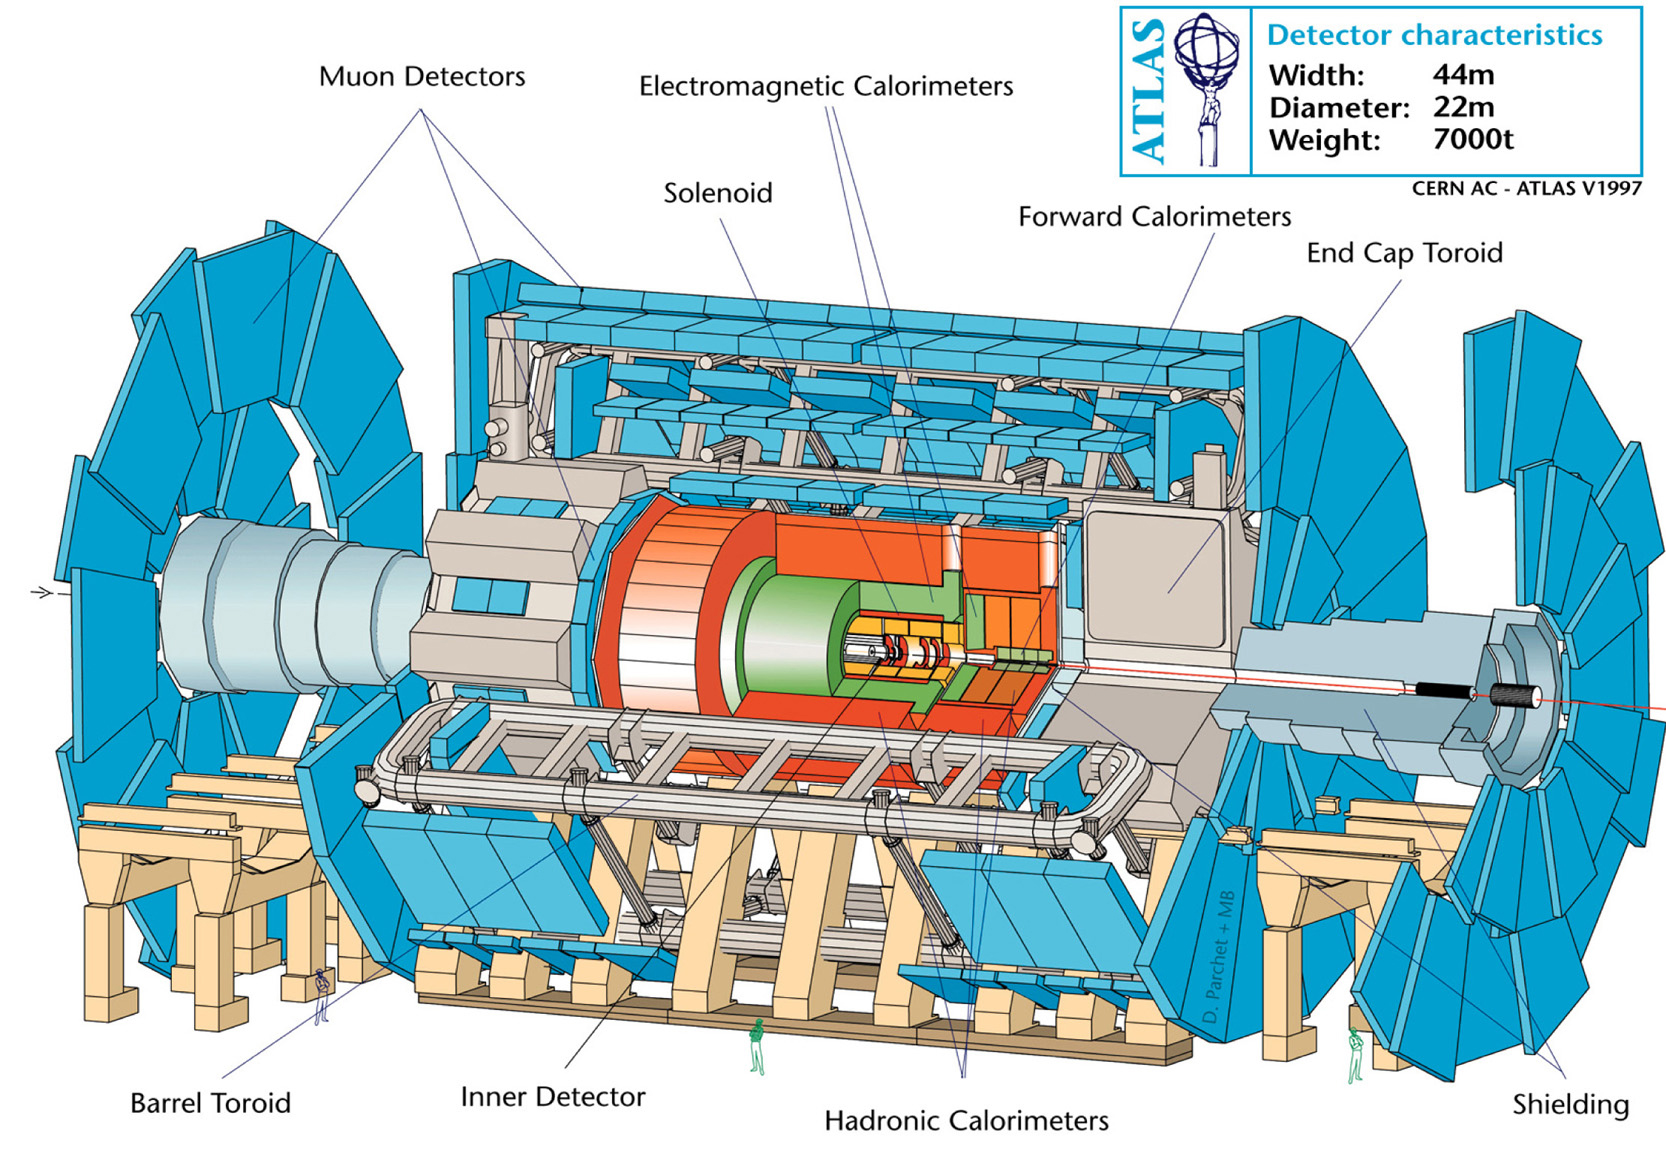
\includegraphics[width=\textwidth]{atlasdet}
	\caption{Current ATLAS detector.}
	\label{fig:current_atlasdet}
\end{figure}

This section briefly describes the current experimental apparatus, shown in Figure \ref{fig:current_atlasdet}, and the reasons as to why it cannot withstand the conditions of HL-LHC.
\smallskip
ATLAS detector is currently composed by the following components:
\begin{itemize}
\item a \textbf{magnet system}
\item an \textbf{inner detector}
\item an \textbf{electromagnetic calorimeter}
\item an \textbf{hadronic calorimeter}
\item a \textbf{muon spectrometer}
\item a \textbf{trigger system}
\item a \textbf{data acquisition system (DAQ)}
\end{itemize}

In the following sections these elements are briefly described, outlining the main upgrades that will be applied. 

\subsection{The magnet system}\label{sec:magnet}

\begin{figure} [h]
	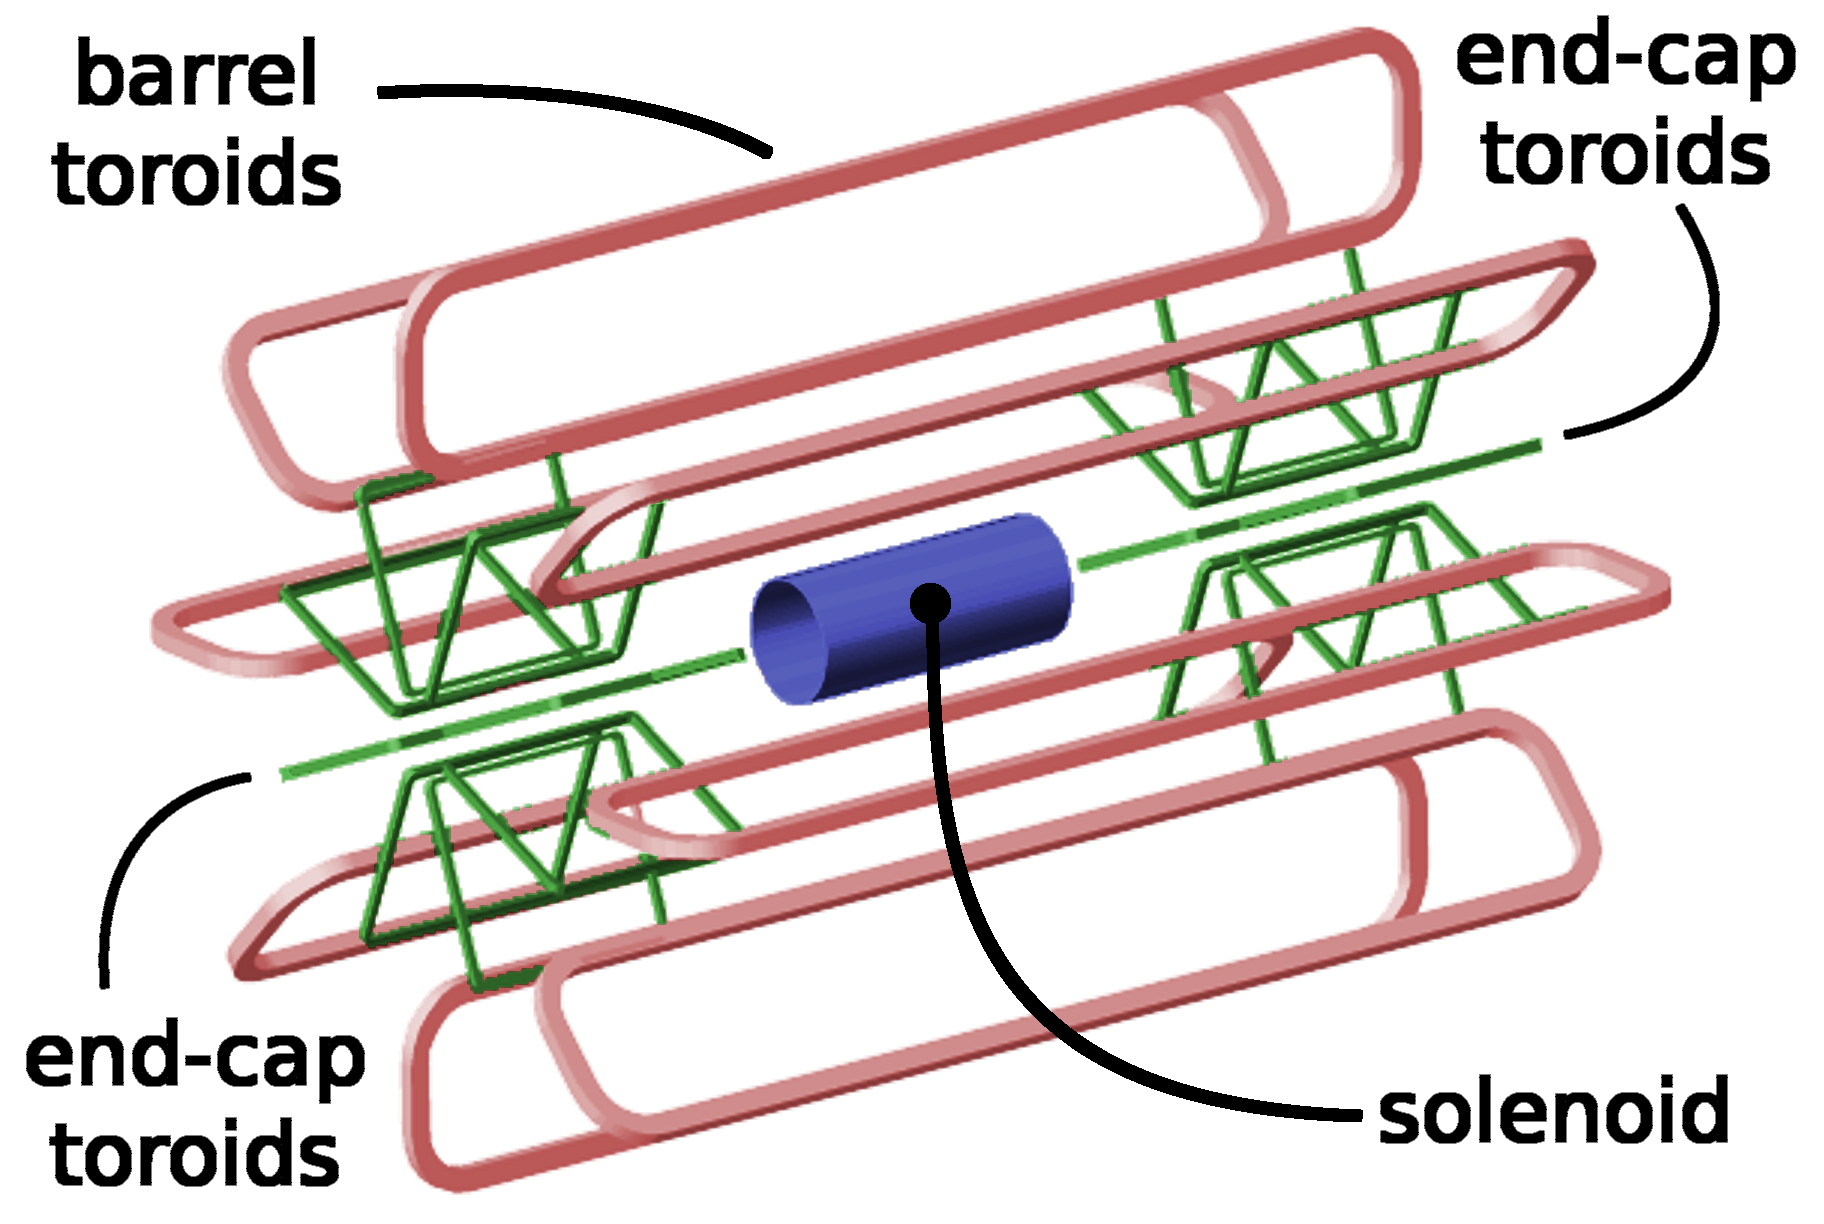
\includegraphics[width=\textwidth]{magnetSystems}
	\caption{ATLAS magnet system\cite{magnet_system_picture}.}
	\label{fig:magnet_system_picture}
\end{figure}

The current magnet system (Fig.\ref{fig:magnet_system_picture}) comprises four superconducting magnets\cite{magnetic_system}, for charged particles bending and momentum measurement in the $8000\ m^3$ volume of the apparatus.\\[2pt]
The Central Solenoid magnet encloses the tracking volume and provides a $2\ T$ magnetic field and minimal thickness in order to reduce the degradation of photon and electron energy resolution in the subsequent calorimeter layers.\\[2pt]
The Barrel and Endcap Toroids provides a tangential magnetic field of about $1\ T$ for the muon detectors, both in the radial and the forward region.\\[2pt]
As the current magnet system already fulfils HL-LHC requirements, it is not going to be
upgraded during that phase. [ref? NON SE NE PARLA NEL LOI/SCOPING]

\subsection{The Inner Detector}

\subsection{The Calorimeter System}

ATLAS experiment  relies on an electromagnetic and an hadronic calorimeter for the identification and the measurement of physical quantities of photons, electrons, hadrons and jets. 
Both compartments are divided into a central and a forward region (Fig.\ref{fig:current_Cals}).

\begin{figure} [h]
	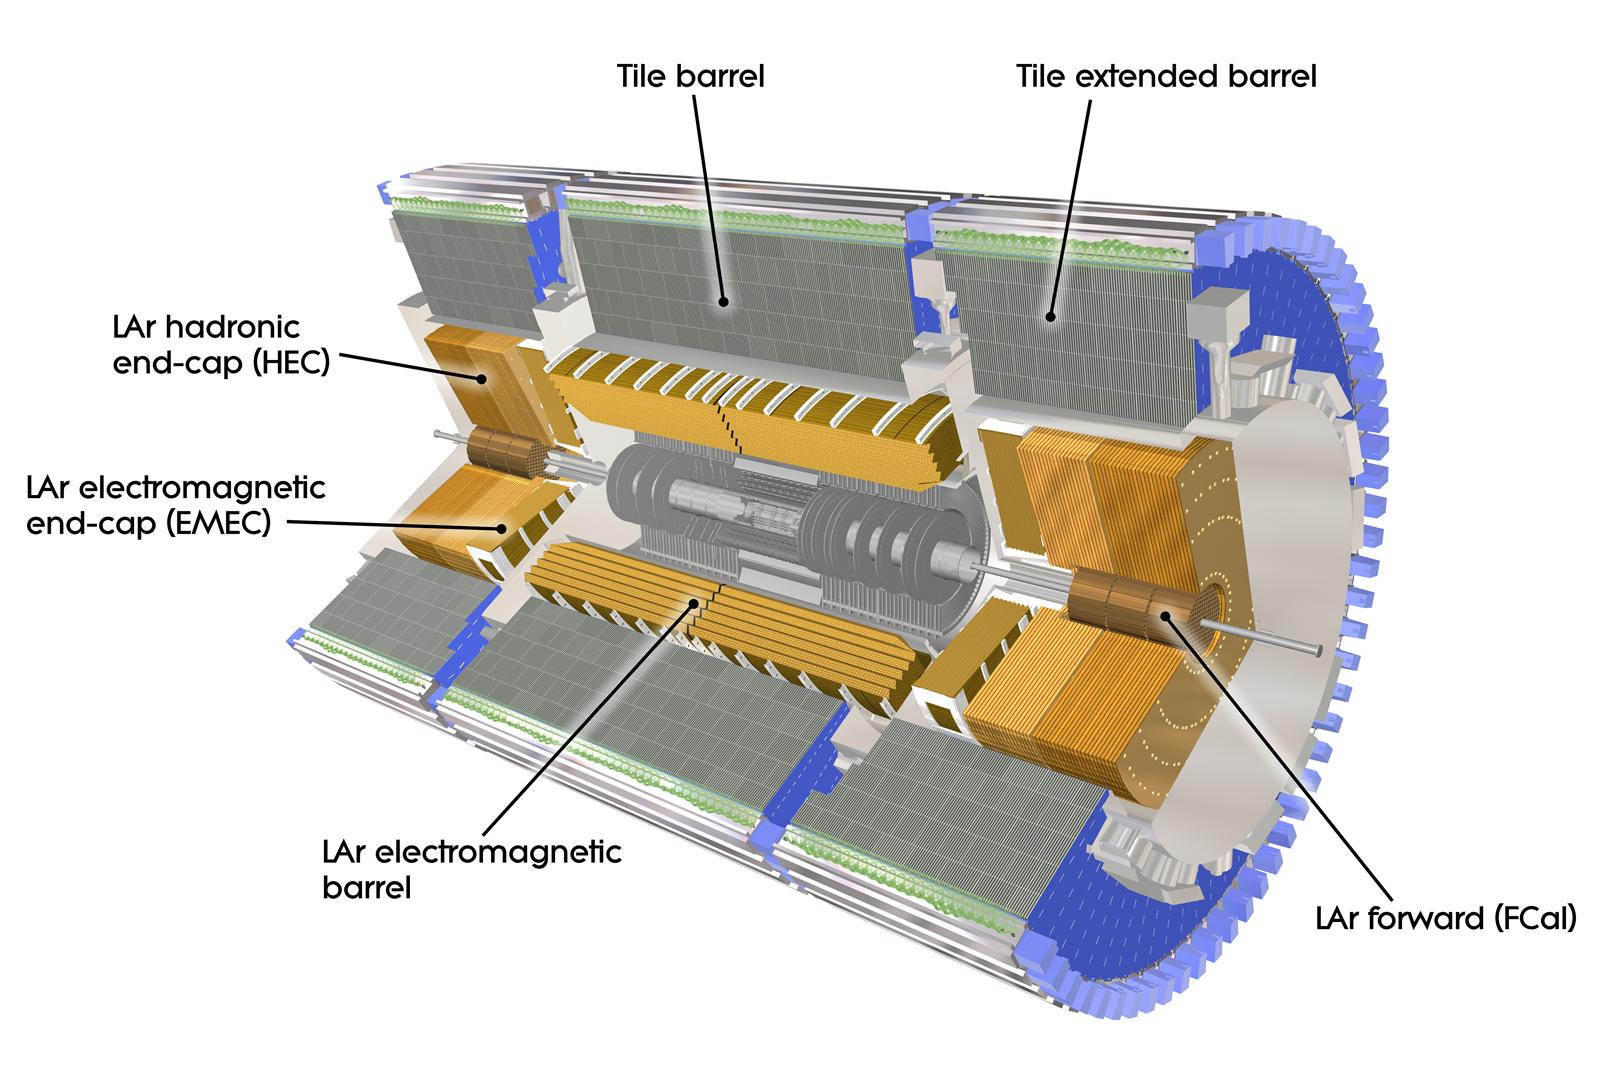
\includegraphics[width=\textwidth]{current_Cals}
	\caption{ATLAS Calorimeter System.}
	\label{fig:current_Cals}
\end{figure}

\subsubsection{Liquid Argon Calorimeters}\label{sec:LAr}
Several calorimeters in ATLAS use liquid Argon (LAr) as active medium\cite{current_ELCal}. The electromagnetic barrel and endcap (EMEC) are entirely made up this way, but also the Hadronic Endcap Calorimeter (HEC) and the Forward Calorimeter (FCal). \\[2pt]
The \textbf{electromagnetic calorimeter} uses lead as absorber and is designed to trigger on and to provide precision measurements of electrons, photons, jets, and missing $E_T$ .
The full cryostat of the \textit{barrel section} is $6.8\ m$ long, with the inner and outer radius being respectively $1.15\ m$ and $2.25\ m$ and ranges in $|\eta|$ from 0 to 1.7.  The \textit{endcap section} is made up of two concentric wheels, the larger one ranging in $|\eta|$ from 1.4 to 2.5, the smaller from 2.5 to 3.2. In addition, a \textit{presampler} layer has been inserted behind the cryostat wall to allow measurement correction due to losses in the upstream material. The amount of inactive material due to the solenoid
accounts for $0.63\ X_0$ and, as cited in Sec.\ref{sec:magnet}, has been optimized. As suggested from detailed simulations based on the response to high energy photons and electrons, the thickness of the calorimeter is about $24\ X_0$ in the barrel and $26\ X_0$ in the endcap. Each section is physically divided into towers which produce the signal and are so responsible
for the granularity of the calorimeter.
High granularity is especially required in the central regions, where it reaches the value of 
$\Delta\eta\ \times\ \Delta\phi\ =\ 0.025\ \times\ 0.025$. In this region is possible to combine the signal of the calorimeter with the information coming from the inner detector to improve the rejection power of $\pi_0$ against photons. Indeed, granularity is less and less relevant to the overall performance with increasing $|\eta|$. Hermeticity is also important for the measurement of missing $E_T$ and has been maximized using a transition gap between the barrel and endcap cryostats of 95 mm. \\[2pt]

\textbf{HEC}\cite{hec} is a sampling calorimeter with copper absorber plates and consists of two wheels of outer radius $2.03\ m$, made of 32 identical modules. It ranges in $|\eta|$ from 1.4 to 3.2 and every half of it shares the cryostat with the EMEC and FCal. \\[2pt]

\textbf{FCal} has to cope with a high level of radiation, which makes it a particularly challenging detector. To avoid an excessive neutron albedo in the central cavity the detector is actually recessed by 
$1.2\ m$ with respect to the frontal face of the electromagnetic calorimeter. FCal is a high density mixed copper-tungsten calorimeter and covers the range of $3.0\ < |\eta|\ <\ 4.9$.  The high density allows to reach the required $9.5\ \lambda$ in a reduced space and to minimize the endcap calorimeter pileup signal.  \\[2pt]

The performance required by HL-LHC barrel electromagnetic calorimeter is the same as the current one, thus it does not need to be upgraded. In contrast to that, the FCal performances will be degraded by the conditions of HL-LHC. That said, the Reference Scenario of the ATLAS Scoping Document\cite{scoping} foresees the replacement of current FCal with a high-granularity Small-Gap Forward Calorimeter (sFCal), superior to the current one in terms of resolution and size of LAr gaps. These latter are designed to be smaller than the current, in order to reduce the risk of formation of Argon bubbles, due to the high energy release. (?? This improvement in granularity would be also required by the extension in $|\eta|$ of the Inner Detector in the aforementioned scenario ??). This replacement and the addition of a High Granularity Timing Detector (HGTD), that will be hopefully installed in front of the LAr Calorimeter endcaps and will be needed to reduce the (??OUT-OF-TIME??) pileup signal. It will cover the range $2.4\ <\ |\eta|\ <\ 4.3$ and it will measure the arrival time of charged particles, assigning them to different collision vertices. The readout electronics will also need to be exchanged due to insufficient radiation tolerance and poor performance with respect to that necessary for the foreseen trigger upgrade. In the Middle and Low cost 
scenarios, on the contrary, no upgrades in the endcap and forward region are foreseen, unless the risk of formation of Argon bubbles is considered too high, in which case a MiniFCal will be installed in front of the existing FCal. 

\subsubsection{Hadron Tile calorimeters}
The \textbf{Tile calorimeter} is a sampling calorimeter composed by alternated layers of scintillating tiles as active medium and steel as an absorber. The signal is carried out from each module using optical fibres, which can run through the layers thanks to the laminated structure of the calorimeter. It is segmented, thus providing a resolution of
$\Delta\eta \times \Delta\phi\ = 0.1 \times 0.1$.\\
The Tile Calorimeter is made up of one barrel ($5.64\ m$ long) and two extended barrel ($2.91\ m$ long) parts, with a gap of $60\ cm$ in between. It consists of a cylindrical structure of inner radius $2.28\ m$ and $4.23\ m$. The barrel covers the region $0\ <\ |\eta|\ <\ 1.0$ whereas the extended covers the region $0.8\ <\ |\eta|\ <\ 1.7$. The overlap region from 0.8 to 1.0 is
occupied by an Intermediate Tile Calorimeter (ITC).\\
The main requirement for the Tile Calorimeter is to reconstruct the energy of the jets produced in the collisions and, due to the high center-of-mass energy at LHC, it has to assure 
high performances in a wide range of energies. Thanks to the use of an extended barrel, the HEC and the FCal (see Sec.\ref{sec:LAr}), it provides a good $p_T^{miss}$ reconstruction.\\[2pt]

The Tile Calorimeter maintains the required performance even during the HL-LHC phase and
so it does not need replacement. On the contrary, the readout electronics will need to be upgraded due to limited radiation tolerance and to accommodate the new trigger requirements in terms of rates and latencies. This will be fulfilled, as in the case of the LAr (see
Section \ref{sec:LAr}), by substituting the on-detector front-end electronics, the optical links, the off-detector signal processing unit, the powering system and the interface modules to the TTC and DAQ systems. (??).

\subsection{Muon Spectrometer}\label{sec:muon}\cite{muon_tdr}\cite{Aad:2008zzm}

\begin{figure} [h]
	\centering
	\includegraphics[scale=0.4]{muonSystem}
	\caption{ATLAS Muon System\cite{muon_tdr}.}
	\label{fig:muonSystem}
\end{figure}

ATLAS \textbf{muon spectrometer} is designed to track charged particles that manage to pass through the whole calorimetric system and to perform stand-alone measurements of their momentum, in the range 
$3\ GeV < p_{T} < 3\ TeV$. Even at the upper limit, the detector is still able to provide adequate momentum resolution and charge sign measurement.\\

The layout of the current  ATLAS muon spectrometer is shown if Fig. \ref{fig:muonSystem}. It is divided into three main regions of pseudorapidity: in the range $0.0 < |\eta| < 1.0$ the bending power
is provided by a barrel magnet composed by eight coils; the range $1.4 < |\eta| < 2.7$ is, instead, covered by a pair of \textit{end-cap toroids} placed at the tips of the barrel toroid; the \textit{transition
region}, $1.0 < |\eta| < 1.4$, is covered by a combination of the two. The system is built so that it provides a field that is mostly orthogonal to the particle direction while minimizing the contribution to multiple scattering. A \textit{trigger system} is also available for $|\eta| < 2.4$. \\

In the barrel section the tracks are measured by stations arranged in three concentric cylinders (approximatively $5\ m$, $7.5\ m$ and $10\ m$ radius) while in the end-cap and
transition region other three stations are arranged in disks along the z-axis (approximatively at  $|z| = 7.4\ m$, $10.8\ m$, $14\ m$ and $21.5\ m$). An extra disk is added in the transition
region to increase acceptance. A gap in the region $|\eta| < 0.1$ is necessary to allow for services. The layout is designed so that a track coming from the interaction point can traverse only three of the aforementioned stations.
Four different detector technologies are employed in this detector to optimize momentum reconstruction and trigger efficiency in the 
different regions.  \textit{Monitored drift tube chambers}(MDT) are employed in the barrel and endcap regions (except for the innermost endcap layer, where the particle flux is maximum) to provide precise z coordinate measurement in the bending plane. In the innermost endcap layer, instead, \textit{Cathode Strip Chambers}(CSC) are used to provide $R-\phi$ and time measurements. \\

For the muon trigger system, \textit{Resistive Plate Chambers}(RPC) were selected for the barrel region, while \textit{Thin Gap Chambers}(TGC) were selected for transition and endcap regions. Other
than achieving the triggering functionality, they also provide the coordinate on the non-bending plane to the MDTs. 

\subsubsection{Upgrade}\cite{scoping}
During the HL-LHC upgrade, the huge increase in the average number of pileup events leads to a series of difficulties that must be overcome by a corresponding performance improvement.\\

In particular, the innermost endcap layer will be substituted by \textit{New Small Wheels} that combines small strip TGCs and MicroMegas chambers, both for triggering and 
precision tracking. The MDTs, together with the New Small Wheels, should already be able to provide an adequate performance and will not be substituted. Its read-out electronics, instead, will not 
be able to cope with the high hit rate and the new ATLAS L0/L1 trigger scheme, so it will have to be subtituted. The same also applies for the RPCs and TGCs. In the case of RPCs, moreover,
the gas gain will be lowered to ensure safety in the expected high rate environment and protract its life. New RPCs with increased rate capabilities will be instead placed in the innermost barrel layer to maintain a
good trigger efficiency, while new high resolution TGCs will substitute the present ones in the middle endcap disk to keep fake rate at a minimum.\\

The possibility to extend the coverage to $|\eta| < 4$ to identify muons and tag inner detector tracks in that range will be made possible by inserting micro-pattern gaseous or silicon pixel
detectors in the region $2.7 < |\eta| < 4.0$.

\subsection{Trigger and DAQ system}
The current ATLAS \textbf{trigger system} is structured in three levels of event selection. 





\newpage
\section{Conclusions}
\label{Conclusions}
\baselineskip 25pt
\baselineskip 5pt
\baselineskip 16pt

%%% EVENTUALE
\appendix

%%% OBBLIGATORIA:

\bibliographystyle{unsrt}
\bibliography{biblio}

\end{document}
